%----------------------------------------------------------------------------------------
%	PACKAGES AND THEMES
%----------------------------------------------------------------------------------------
\documentclass[aspectratio=169,xcolor=dvipsnames]{beamer}
\usetheme{SimplePlusAIC}
\usefonttheme{professionalfonts}

\usepackage{hyperref}
\usepackage{graphicx} % Allows including images
\usepackage{booktabs} % Allows the use of \toprule, \midrule and  \bottomrule in tables
\usepackage{svg} %allows using svg figures
\usepackage{tikz}
\usepackage{makecell}
\newcommand*{\defeq}{\stackrel{\text{def}}{=}}

\newcommand{\ie}{\textit{\fontspec{Times New Roman}i.e.}}
\newcommand{\eg}{\emph{e.g.}}
\usepackage{natbib}
\usepackage{ulem}
\usepackage{wrapfig}
\usepackage{ragged2e}
\usepackage{bm}
\usepackage[ruled,vlined,linesnumbered]{algorithm2e}
\usepackage{hyperref}



%Select the Epilogue font (requires luaLatex or XeLaTex compilers)
\usepackage{fontspec}
\setsansfont{Epilogue}[
    Path=./epilogueFont/,
    Scale=0.9,
    Extension = .ttf,
    UprightFont=*-Regular,
    BoldFont=*-Bold,
    ItalicFont=*-Italic,
    BoldItalicFont=*-BoldItalic
    ]

%----------------------------------------------------------------------------------------
%	TITLE PAGE
%----------------------------------------------------------------------------------------

\title[short title]{Nonparametric Iterative Machine Teaching} % The short title appears at the bottom of every slide, the full title is only on the title page

\author{Chen Zhang$^1$, Xiaofeng Cao$^1$, Weiyang Liu$^{2,3}$, Ivor W. Tsang$^{4}$, James T. Kwok$^{5}$}
\institute{$^1$Jilin University\newline $^2$Max Planck Institute for Intelligent Systems\newline $^3$University of Cambridge\newline $^4$Agency for Science, Technology and Research \newline $^5$Hong Kong University of Science and Technology}
% Your institution as it will appear on the bottom of every slide, maybe shorthand to save space


\date{\today} % Date, can be changed to a custom date
%----------------------------------------------------------------------------------------
%	PRESENTATION SLIDES
%----------------------------------------------------------------------------------------

\begin{document}

\begin{frame}[plain]
    % Print the title page as the first slide
    \titlepage
\end{frame}

\begin{frame}{Overview}
    % Throughout your presentation, if you choose to use \section{} and \subsection{} commands, these will automatically be printed on this slide as an overview of your presentation
    \tableofcontents
\end{frame}

%------------------------------------------------
\section{What is Machine Teaching?}
%------------------------------------------------

\begin{frame}{What is Machine Teaching?}

\justify
Machine teaching (MT)~\cite{zhu2015machine, zhu2018overview} is the study of how to design the \alert{optimal teaching set}, typically with \alert{minimal} examples, so that learners can quickly learn \alert{target models} based on these examples.
\vspace{1mm}

\justify
It can be considered an \alert{inverse problem} of machine learning, where \uline{machine learning aims to learn model parameters from a dataset}, while \uline{MT aims to find a minimal dataset from the target model parameters}.

\vspace{1mm}

\justify
Considering the \alert{interaction manner} between teachers and learners, MT can be conducted in either\begin{itemize}
    \item {\color{blue} batch} fashion \cite{zhu2015machine, mansouri2019preference, kumar2021teaching, qian2022teaching} where the teacher is allowed to interact with the learner {\color{red} once}, or 
    \item {\color{blue} iterative} fashion \cite{liu2017iterative, liu2018towards, Liu2021LAST} where an iterative teacher would feed examples {\color{red} sequentially} based on current status of the iterative learner.
\end{itemize}

\end{frame}

%------------------------------------------------
\section{Nonparametric Iterative Machine Teaching}
%------------------------------------------------
\begin{frame}{Nonparametric Iterative Machine Teaching}

\justify
Previous iterative machine teaching algorithms \cite{liu2017iterative, liu2018towards, xu2021locality, wang2021gradient} are solely based on \alert{parameterized} families of target models. They mainly focus on convergence in the parameter space, resulting in difficulty when the target models are defined to be \alert{functions without dependency on parameters}. 

\vspace{1mm}

To address such a limitation, we study a more general task -- {\bf Nonparametric Iterative Machine Teaching}, which aims to teach {\color{red} nonparametric target models} to learners in an iterative fashion.

\vspace{-3mm}

\begin{figure}
  \centering
  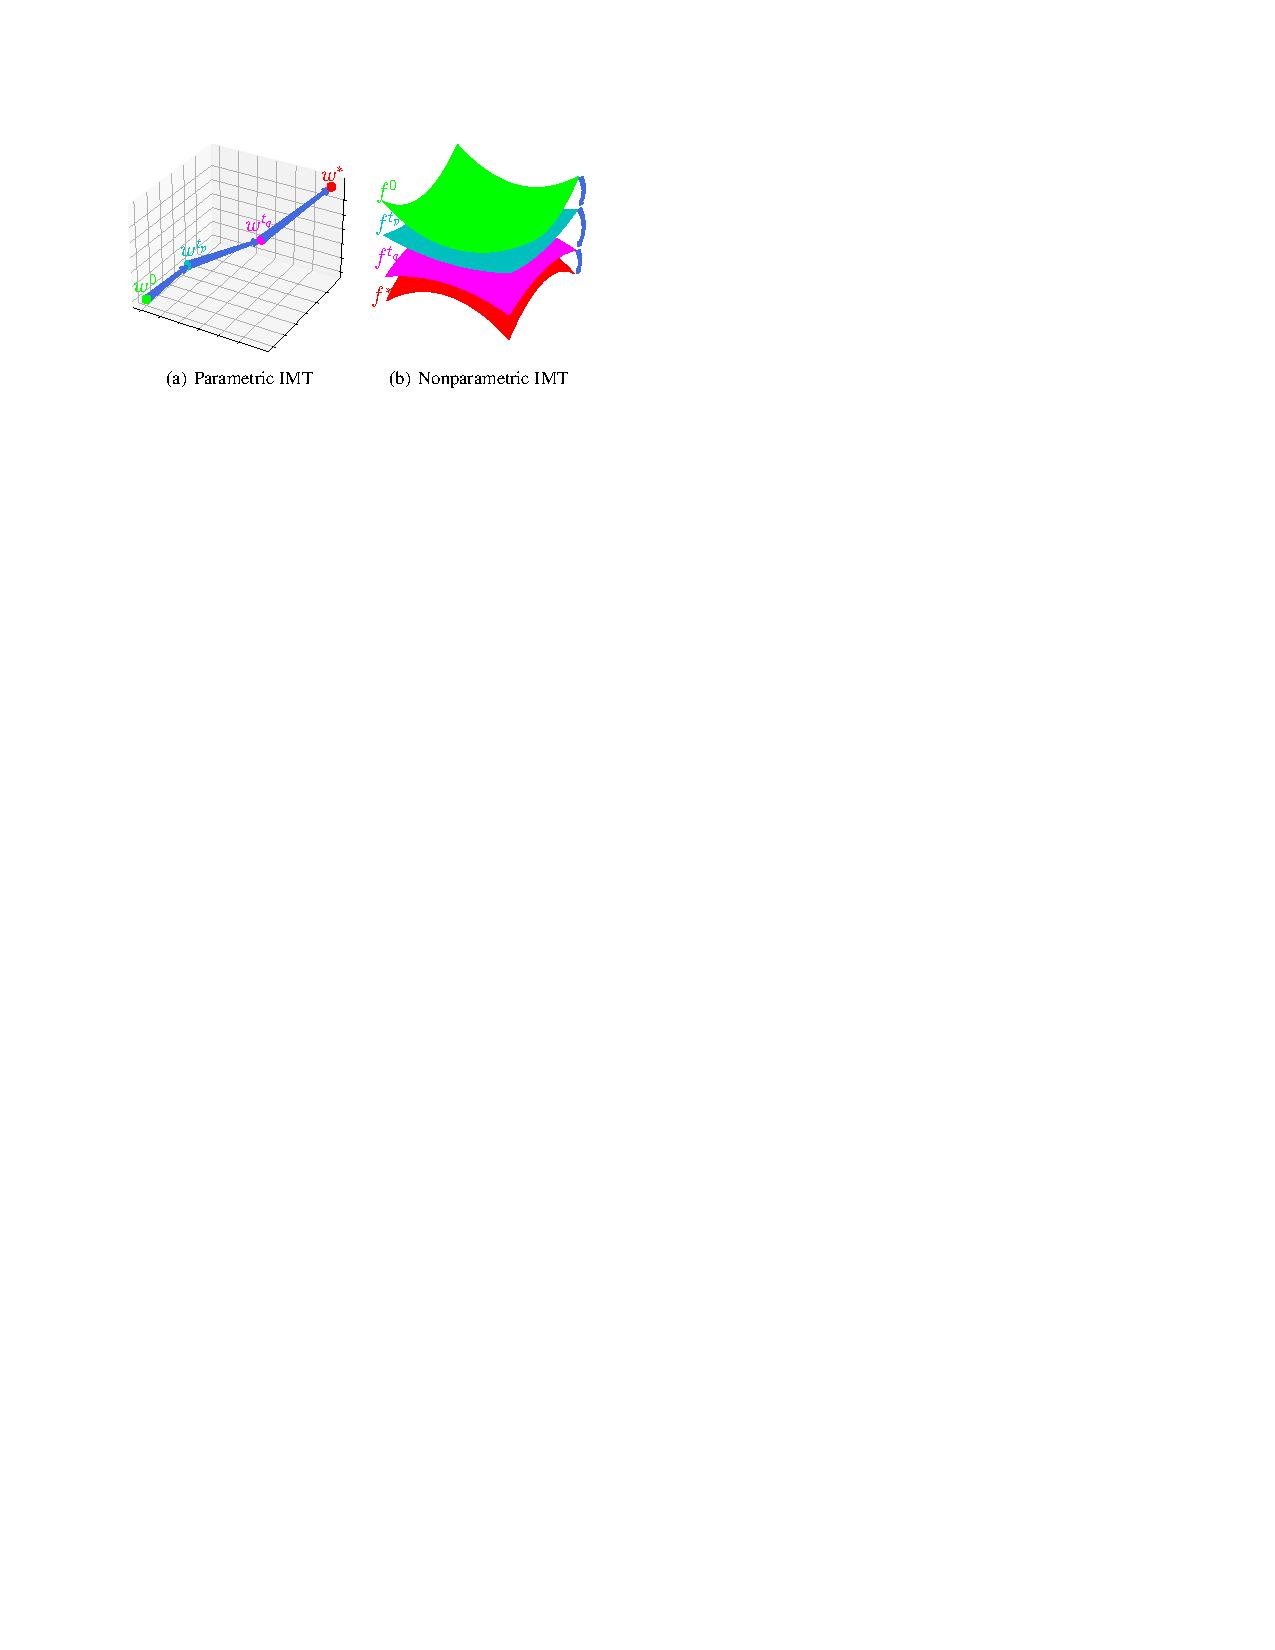
\includegraphics[width=0.45\textwidth]{comp.pdf}
\end{figure}
\end{frame}


\begin{frame}{Cont.}

{\bf \color{blue} Main Contribution}: 
\begin{itemize}
\item We comprehensively study {\bf Nonparametric Iterative Machine Teaching}, which focuses on exploring iterative algorithms for teaching \alert{parameter-free target models} from the \alert{optimization} perspective.
\item We propose two teaching algorithms, which are named \alert{Random Functional Teaching} (RFT) and \alert{Greedy Functional Teaching} (GFT), respectively. RFT is based on random sampling with ground truth labels, and the derivation of GFT is based on the maximization of an informative scalar.
\item We theoretically analyze the \alert{asymptotic behavior} of both RFT and GFT. We prove that per-iteration reduction of loss $\mathcal{L}$ for RFT and GFT has a \alert{negative upper bound} expressed by the discrepancy of iterative teaching, and we derive that the iterative teaching dimension (ITD) of GFT is $\mathcal{O}(\psi(\frac{2\mathcal{L}(f^0)}{\tilde{\eta}\epsilon}))$, which is shown to be lower than the ITD of RFT, $\mathcal{O}(2\mathcal{L}(f^0)/\left(\tilde{\eta}\epsilon\right))$.
\end{itemize}
\end{frame}
%------------------------------------------------
\subsection{Teaching Settings}
\begin{frame}{Teaching Settings}

{\bf \color{blue} Functional Optimization}: We define nonparametric iterative machine teaching as a \alert{functional minimization} over the collection of potential teaching sequences $\mathbb{D}$ in the reproducing kernel Hilbert space:
\begin{equation}\label{eq1}
 \mathcal{D}^*=\underset{\mathcal{D}\in\mathbb{D}}{\arg\min}\quad \mathcal{M}(\hat{f},f^*)+\lambda\cdot \text{len}(\mathcal{D}) \qquad\text{s.t.}\quad\hat{f}=\mathcal{A}(\mathcal{D}),
\end{equation}
where $\mathcal{M}$ denotes a discrepancy measure, $\text{len}(\mathcal{D})$, 
which is regularized by a constant $\lambda$, is the length of the teaching sequence $\mathcal{D}$, and $\mathcal{A}$ represents the learning algorithm of learners. 
\end{frame}


\subsection{Functional Teaching Algorithms}

\begin{frame}{Functional Teaching Algorithms}

\begin{figure}[h]
  \begin{minipage}{0.4\textwidth}
    \begin{figure}
      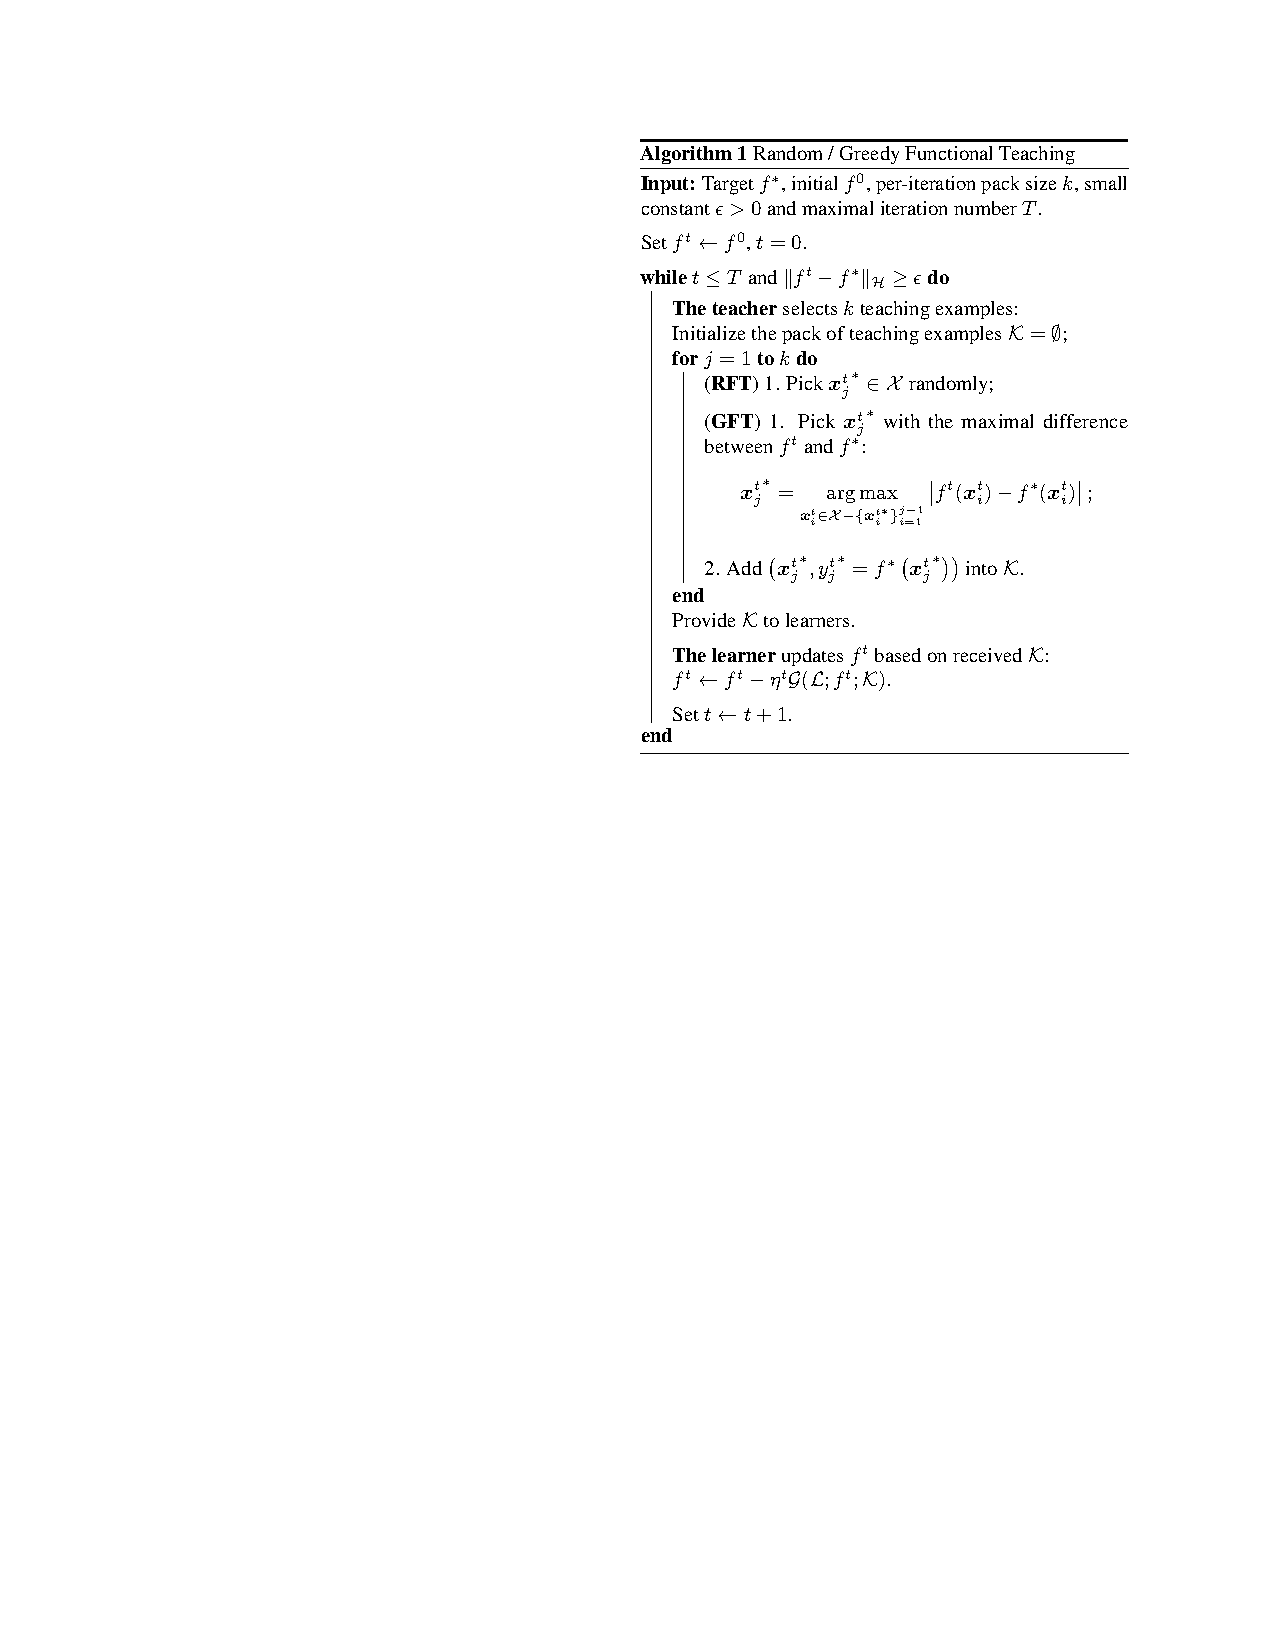
\includegraphics[width=0.92\linewidth]{algo.pdf}
    \end{figure}
  \end{minipage}
  \hfill
  \begin{minipage}{0.55\textwidth} 
    \begin{itemize}
        \item It is straightforward for teachers to pick examples \alert{randomly} and feed them to learners, which derives a simple teaching baseline called \textbf{Random Functional Teaching}.
        \item \textbf{Greedy Functional Teaching} is to search examples with \alert{steeper} gradients, since the gradient norm at the optimal example should be \alert{maximal} at every iteration.
    \end{itemize}

  \end{minipage}
\end{figure}



\end{frame}

%------------------------------------------------
\subsection{Analysis of Iterative Teaching Dimension}
\begin{frame}{Analysis of Iterative Teaching Dimension}

To conduct \textit{theoretical analysis} on the \alert{iterative teaching dimension}, we have listed the assumptions \cite{shen2020sinkhorn} on $\mathcal{L}$ and the kernel function $K(\bm{x},\bm{x}')\in\mathcal{H}$ below.
\begin{block}{Assumption 1}
    The loss function $\mathcal{L}(f)$ is \alert{$L_\mathcal{L}$-Lipschitz smooth}, \ie, $\forall f,f'\in\mathcal{H}$ and $\bm{x}\in\mathcal{X}$ \begin{equation}
        \left|E_{\bm{x}}\left[\nabla_f \mathcal{L}(f)\right]-E_{\bm{x}}\left[\nabla_f\mathcal{L}(f')\right]\right|\leq L_\mathcal{L} \left|E_{\bm{x}}\left[f\right]-E_{\bm{x}}\left[f'\right]\right|,
    \end{equation} where $L_\mathcal{L}\geq0$ is a constant.
\end{block}

\begin{block}{Assumption 2}
The kernel function $K(\bm{x},\bm{x}')\in\mathcal{H}$ is \alert{bounded}, \ie, $\forall \bm{x},\bm{x}' \in\mathcal{X},\,K(\bm{x},\bm{x}')\leq M_K$, where $M_K\geq0$ is a constant.
\end{block}
\end{frame}

\begin{frame}{Cont. (RFT)}
\begin{block}{Lemma (Sufficient Descent for RFT)} Under Assumption 1 and 2, if $\eta^t\leq 1/(2L_\mathcal{L}\cdot M_K)$, RFT teachers can \alert{reduce the loss} $\mathcal{L}$ by $\mathcal{L}(f^{t+1})-\mathcal{L}(f^t)\leq-\eta^t/2\cdot\mathbb{S}_{\mathcal{L}}(f^t;{\bm{x}^t})$.
\end{block}
\begin{theorem}[Convergence for RFT]
        Suppose the model of learners is initialized with $f^0\in\mathcal{H}$ and returns $f^t\in\mathcal{H}$ after $t$ iterations, we have the \alert{upper bound of minimal $\mathbb{S}_{\mathcal{L}}(f^t;{\bm{x}^t})$} as $\min_t\mathbb{S}_{\mathcal{L}}(f^t;{\bm{x}^t}) \leq2\mathcal{L}(f^0)/\left(\tilde{\eta}t\right)$,
	where $0<\tilde{\eta}=\underset{t}{\min}\,\eta^t\leq \frac{1}{2L_\mathcal{L}\cdot M_K}$.
\end{theorem}    
\end{frame}

\begin{frame}{Cont. (GFT)}
\begin{block}{Lemma (Sufficient Descent for GFT)} Under Assumption 1 and 2, if $\eta^t\leq 1/(2L_\mathcal{L}\cdot M_K)$, GFT teachers can reduce the loss $\mathcal{L}$ at a \alert{faster speed}, 
$\mathcal{L}(f^{t+1})-\mathcal{L}(f^t)\leq-\eta^t/2\cdot\mathbb{S}_{\mathcal{L}}(f^t;{\bm{x}^t}^*)\leq-\eta^t/2\cdot\mathbb{S}_{\mathcal{L}}(f^t;{\bm{x}^t})$.
\end{block}
\begin{theorem}[Convergence for GFT]
        Suppose the model of learners is initialized with $f^0\in\mathcal{H}$ and returns $f^t\in\mathcal{H}$ after $t$ iterations, we have the \alert{upper bound of minimal $\mathbb{S}_{\mathcal{L}}(f^t;{\bm{x}^j}^*)$} as $\min_j\mathbb{S}_{\mathcal{L}}(f^j;{\bm{x}^j}^*)\leq\frac{2}{\tilde{\eta}\psi(t)}\mathcal{L}(f^0)$, where $0<\tilde{\eta}=\underset{t}{\min}\,\eta^t\leq \frac{1}{2L_\mathcal{L}\cdot M_K}$, $\psi(t)=\sum_{j=0}^{t-1}\gamma^j$ and $\gamma^j = \frac{\mathbb{S}_{\mathcal{L}}(f^j;{\bm{x}^j})}{\mathbb{S}_{\mathcal{L}}(f^j;{\bm{x}^j}^*)}\in(0,1]$ named greedy ratio.
\end{theorem}    
\end{frame}

%------------------------------------------------
\section{Experiments and Results}
\begin{frame}{Experiments and Results}

\justify
We test our RFT and GFT on both \alert{synthetic} and \alert{real-world} data, on which we find these two algorithms present satisfactory capability to tackle \alert{nonparametric teaching tasks}.

\vspace{1mm}
\begin{itemize}
    \item {\bf Synthetic data.}
\end{itemize}

\centering
\begin{tabular}{lclc}
{\scriptsize \color{blue} 1D Gaussian Mixture.} \vspace{-1.2mm}\\

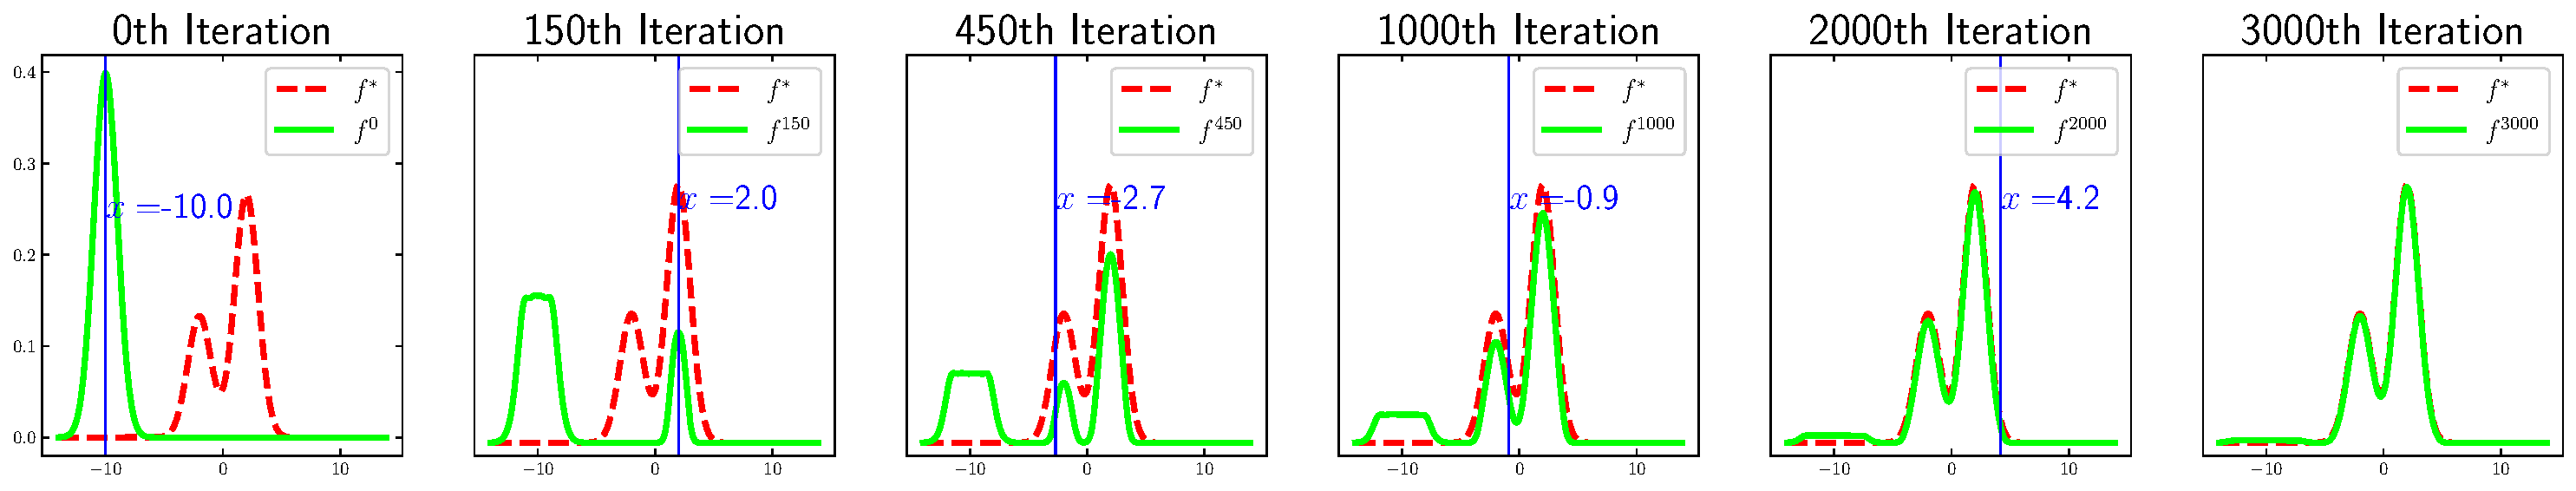
\includegraphics[width=0.8\linewidth]{./out/toy/distribution}\vspace{-1.2mm}\\


{\scriptsize \color{blue} 2D Classification.}\vspace{-1.2mm}\\

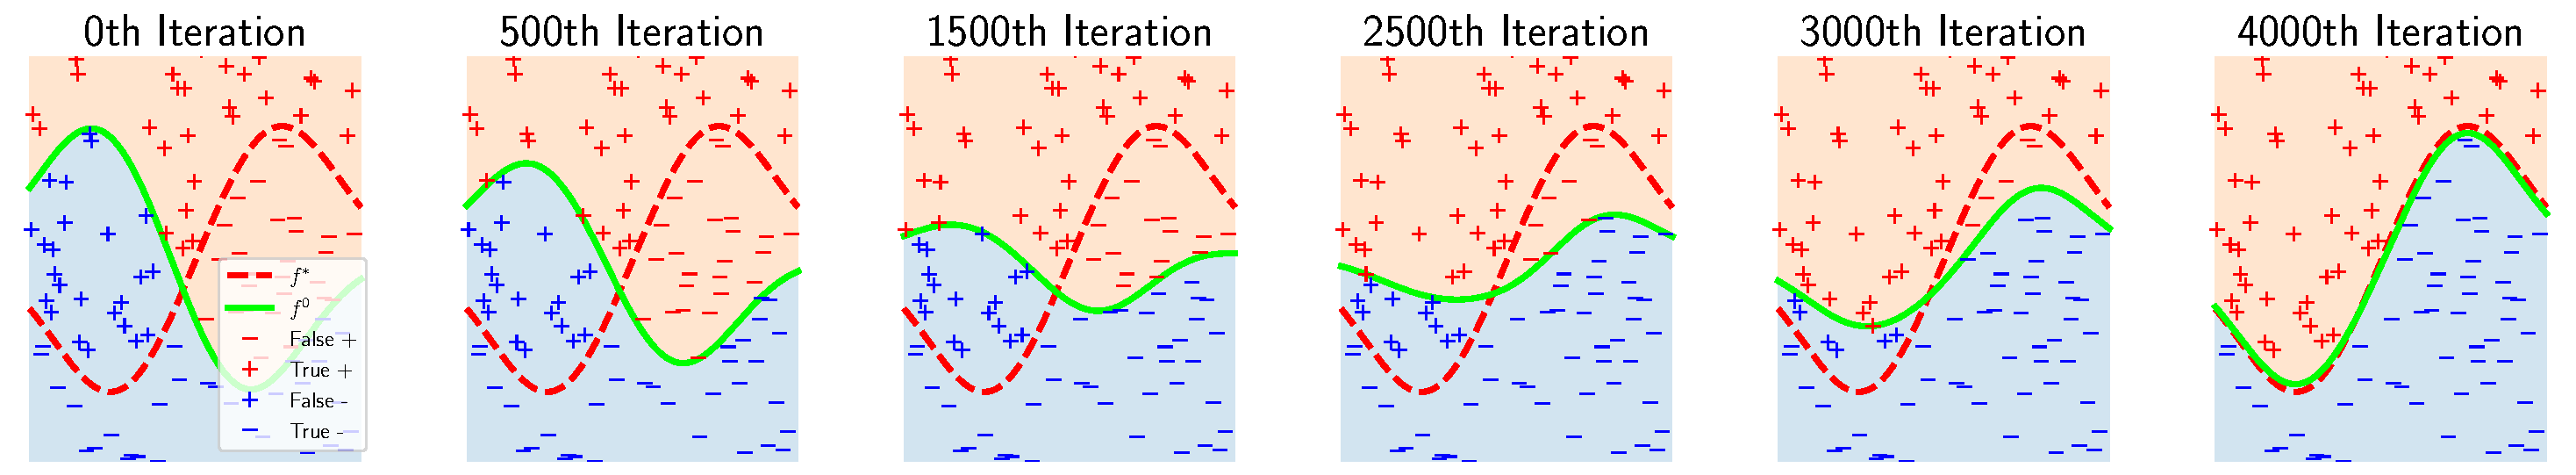
\includegraphics[width=0.8\linewidth]{./out/toy/classification}
\end{tabular}

\end{frame}


\begin{frame}{Cont.}
\begin{itemize}
    \item {\bf  Real-world data.}
\end{itemize}

\centering
\begin{tabular}{ccc}

{\scriptsize \color{blue} Digit Correction.} & & {\scriptsize \color{blue} Cheetah Impartation.}\vspace{-0.8mm}\\

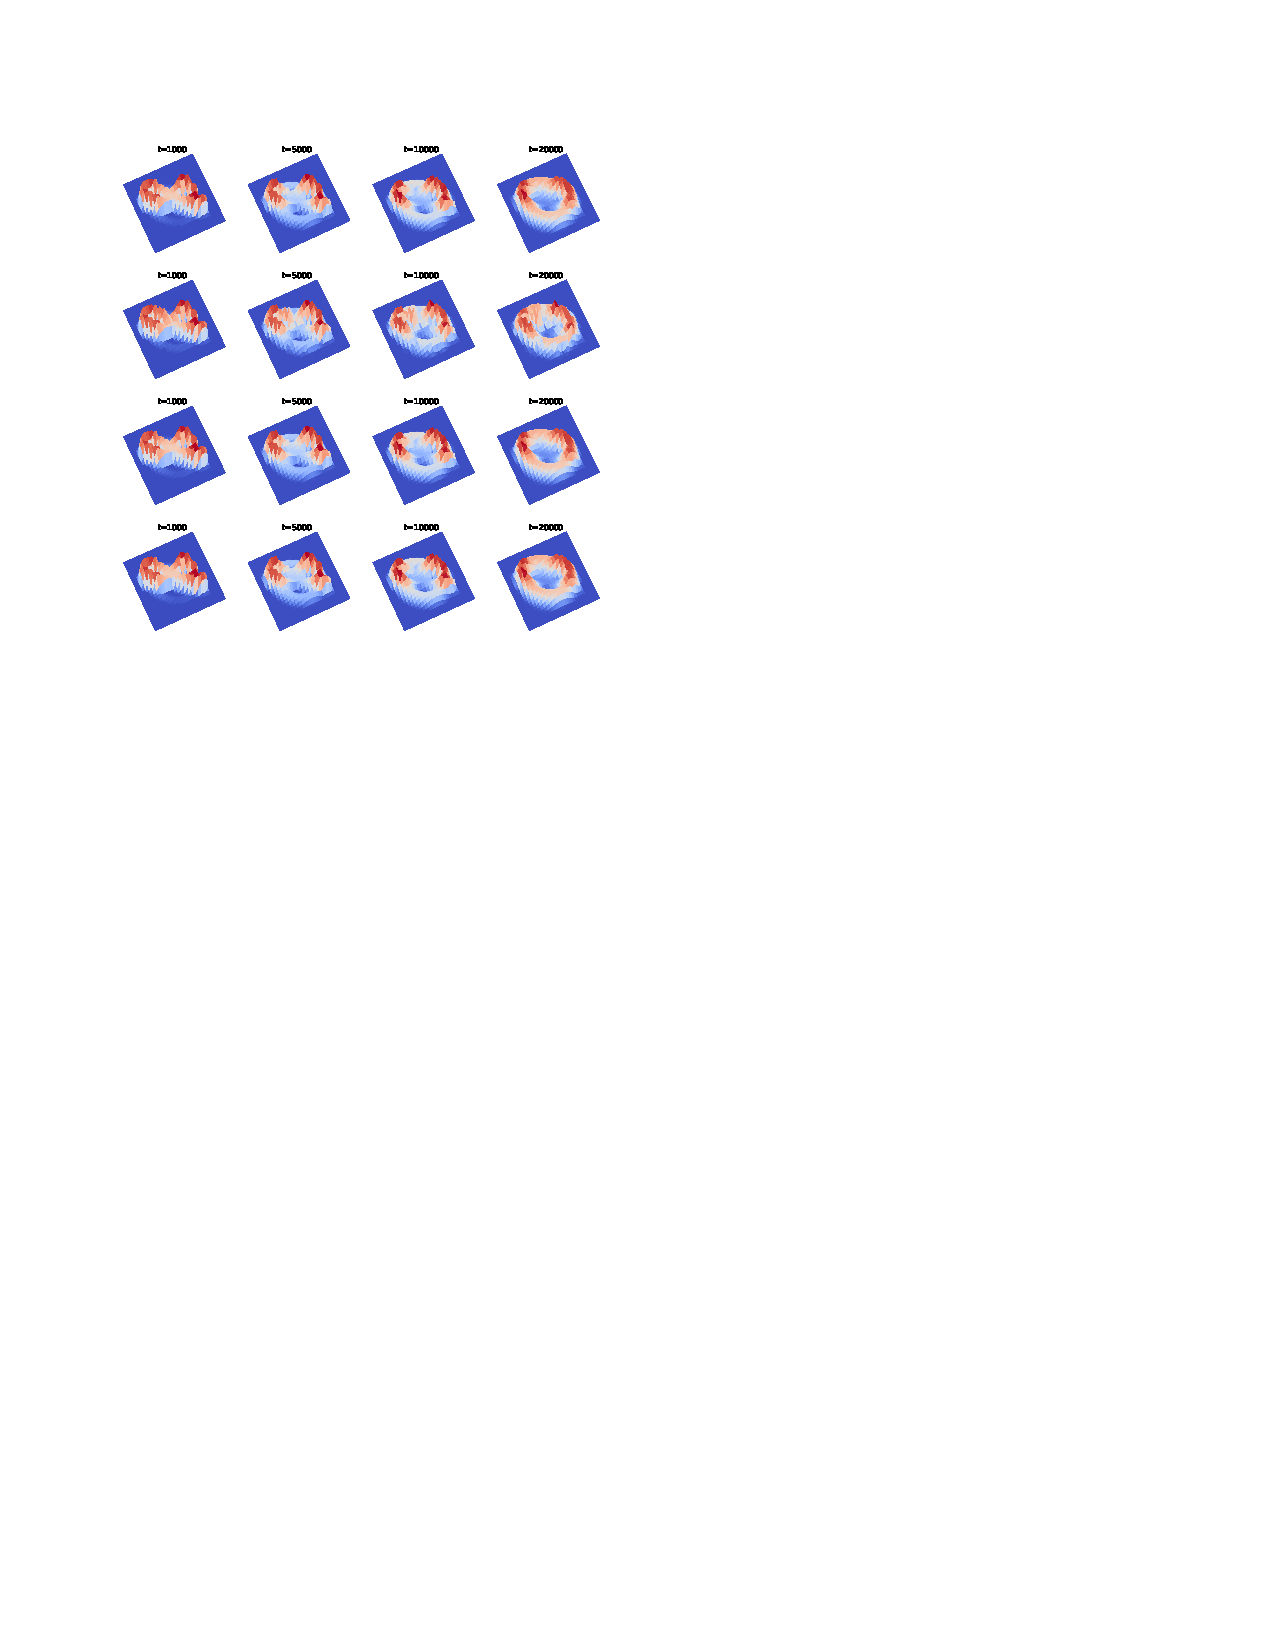
\includegraphics[scale=0.7]{./out/realworld/digit} & 

&
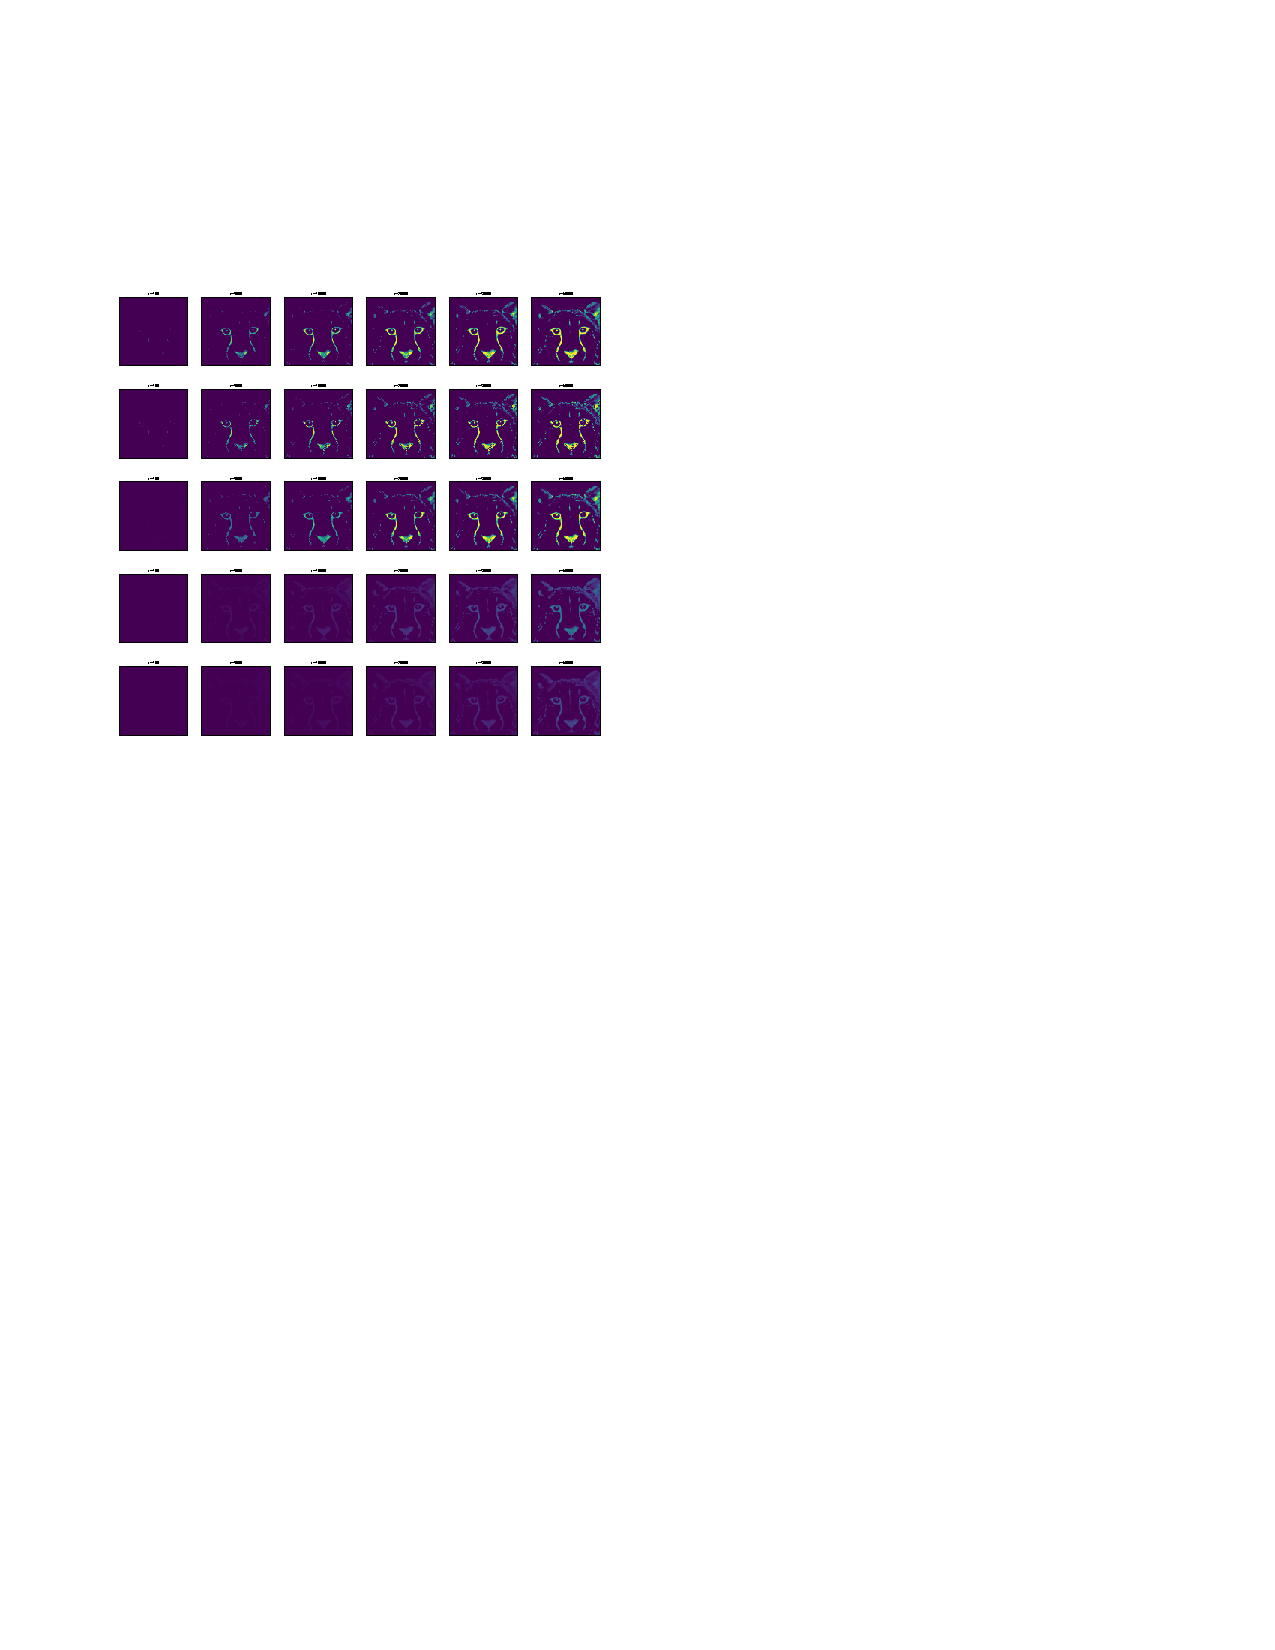
\includegraphics[scale=0.78]{./out/realworld/cheetah}
\end{tabular}

\end{frame}


\begin{frame}{Cont.}
\begin{tabular}{lc}
{\scriptsize \color{blue} Sketch for Missing Person Report.}\vspace{-.8mm}\\

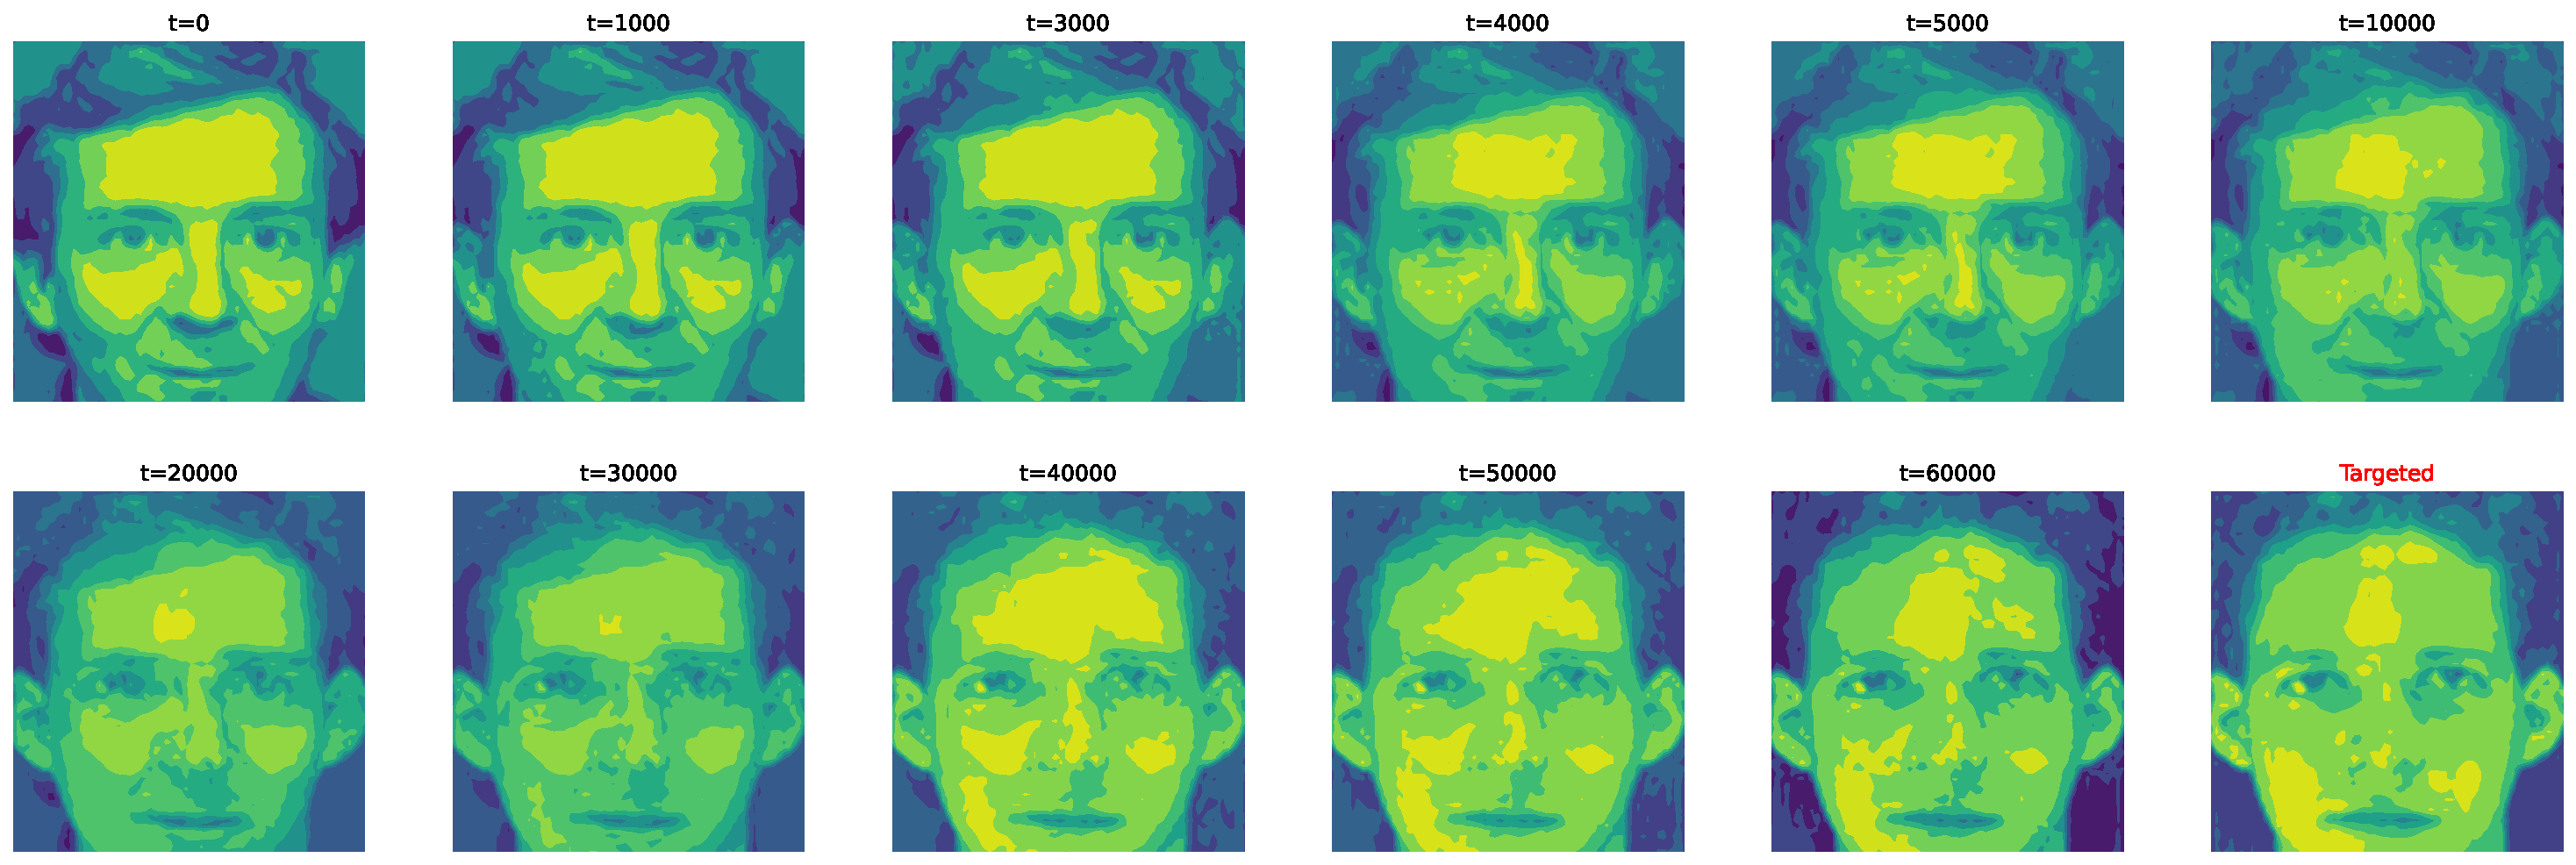
\includegraphics[width=\linewidth]{./out/realworld/2d face eta=0.05 B=one}

\end{tabular}
\end{frame}

%------------------------------------------------
\begin{frame}[allowframebreaks]
    \frametitle{References}
    \bibliographystyle{plain}
    {\footnotesize \bibliography{ref.bib}}
\end{frame}

%------------------------------------------------

\begin{frame}
    \Huge{\centerline{\textbf{Thank you for listening!}}}
\end{frame}

%----------------------------------------------------------------------------------------
\end{document}